\documentclass[aspectratio=169]{beamer}
\useoutertheme[progressbar=frametitle]{metropolis}
\useinnertheme{metropolis}
\definecolor{nabgray}{rgb}{0.6,0.59,0.61}
\usecolortheme[named=nabgray]{structure}
\usepackage{tikz}
\usepackage[utf8]{inputenc}
\usepackage[spanish]{babel}
\usepackage{fontspec}
\setmonofont{JetBrains Mono}
\setmainfont{Roboto}
\setsansfont{Roboto}

\usepackage{smartdiagram}
\usepackage{qtree}
\usepackage{verbatim}
\usepackage{svg}
\usepackage{graphicx}
\usepackage{color}
\definecolor{lightgray}{rgb}{0.95, 0.95, 0.95}
\definecolor{darkgray}{rgb}{0.4, 0.4, 0.4}
\definecolor{ocherCode}{rgb}{1, 0.5, 0} % #FF7F00 -> rgb(239, 169, 0)
\definecolor{blueCode}{rgb}{0, 0, 0.93} % #0000EE -> rgb(0, 0, 238)
\definecolor{greenCode}{rgb}{0, 0.6, 0} % #009900 -> rgb(0, 153, 0)

\usepackage{upquote}
\usepackage{listings}
\lstset{language=java,
    otherkeywords={var,record},
	% Basic design
	backgroundcolor=\color{lightgray},
	basicstyle={\small\ttfamily},
	frame=l,
	keywordstyle=\footnotesize\color{blue},
	escapeinside={<@}{@>},
	breaklines=true,
	% Line numbers
	xleftmargin={0.75cm},
	numbers=left,
	stepnumber=1,
	firstnumber=1,
	numberfirstline=true
	% Code design
	identifierstyle=\color{black},
	keywordstyle=\color{ocherCode}\bfseries,
	ndkeywordstyle=\color{greenCode}\bfseries,
	stringstyle=\color{ocherCode}\ttfamily,
	commentstyle=\color{darkgray}\ttfamily,
	tabsize=2,
	showtabs=true,
	showspaces=false,
	showstringspaces=false,
	extendedchars=true,
	breaklines=true
}

\lstdefinelanguage{bash}{
    basicstyle=\ttfamily,
    showstringspaces=false,
    commentstyle=\color{red},
    keywordstyle=\color{blue},
    numbers=right,
    xleftmargin={0.25cm}
}

\usebackgroundtemplate
{
	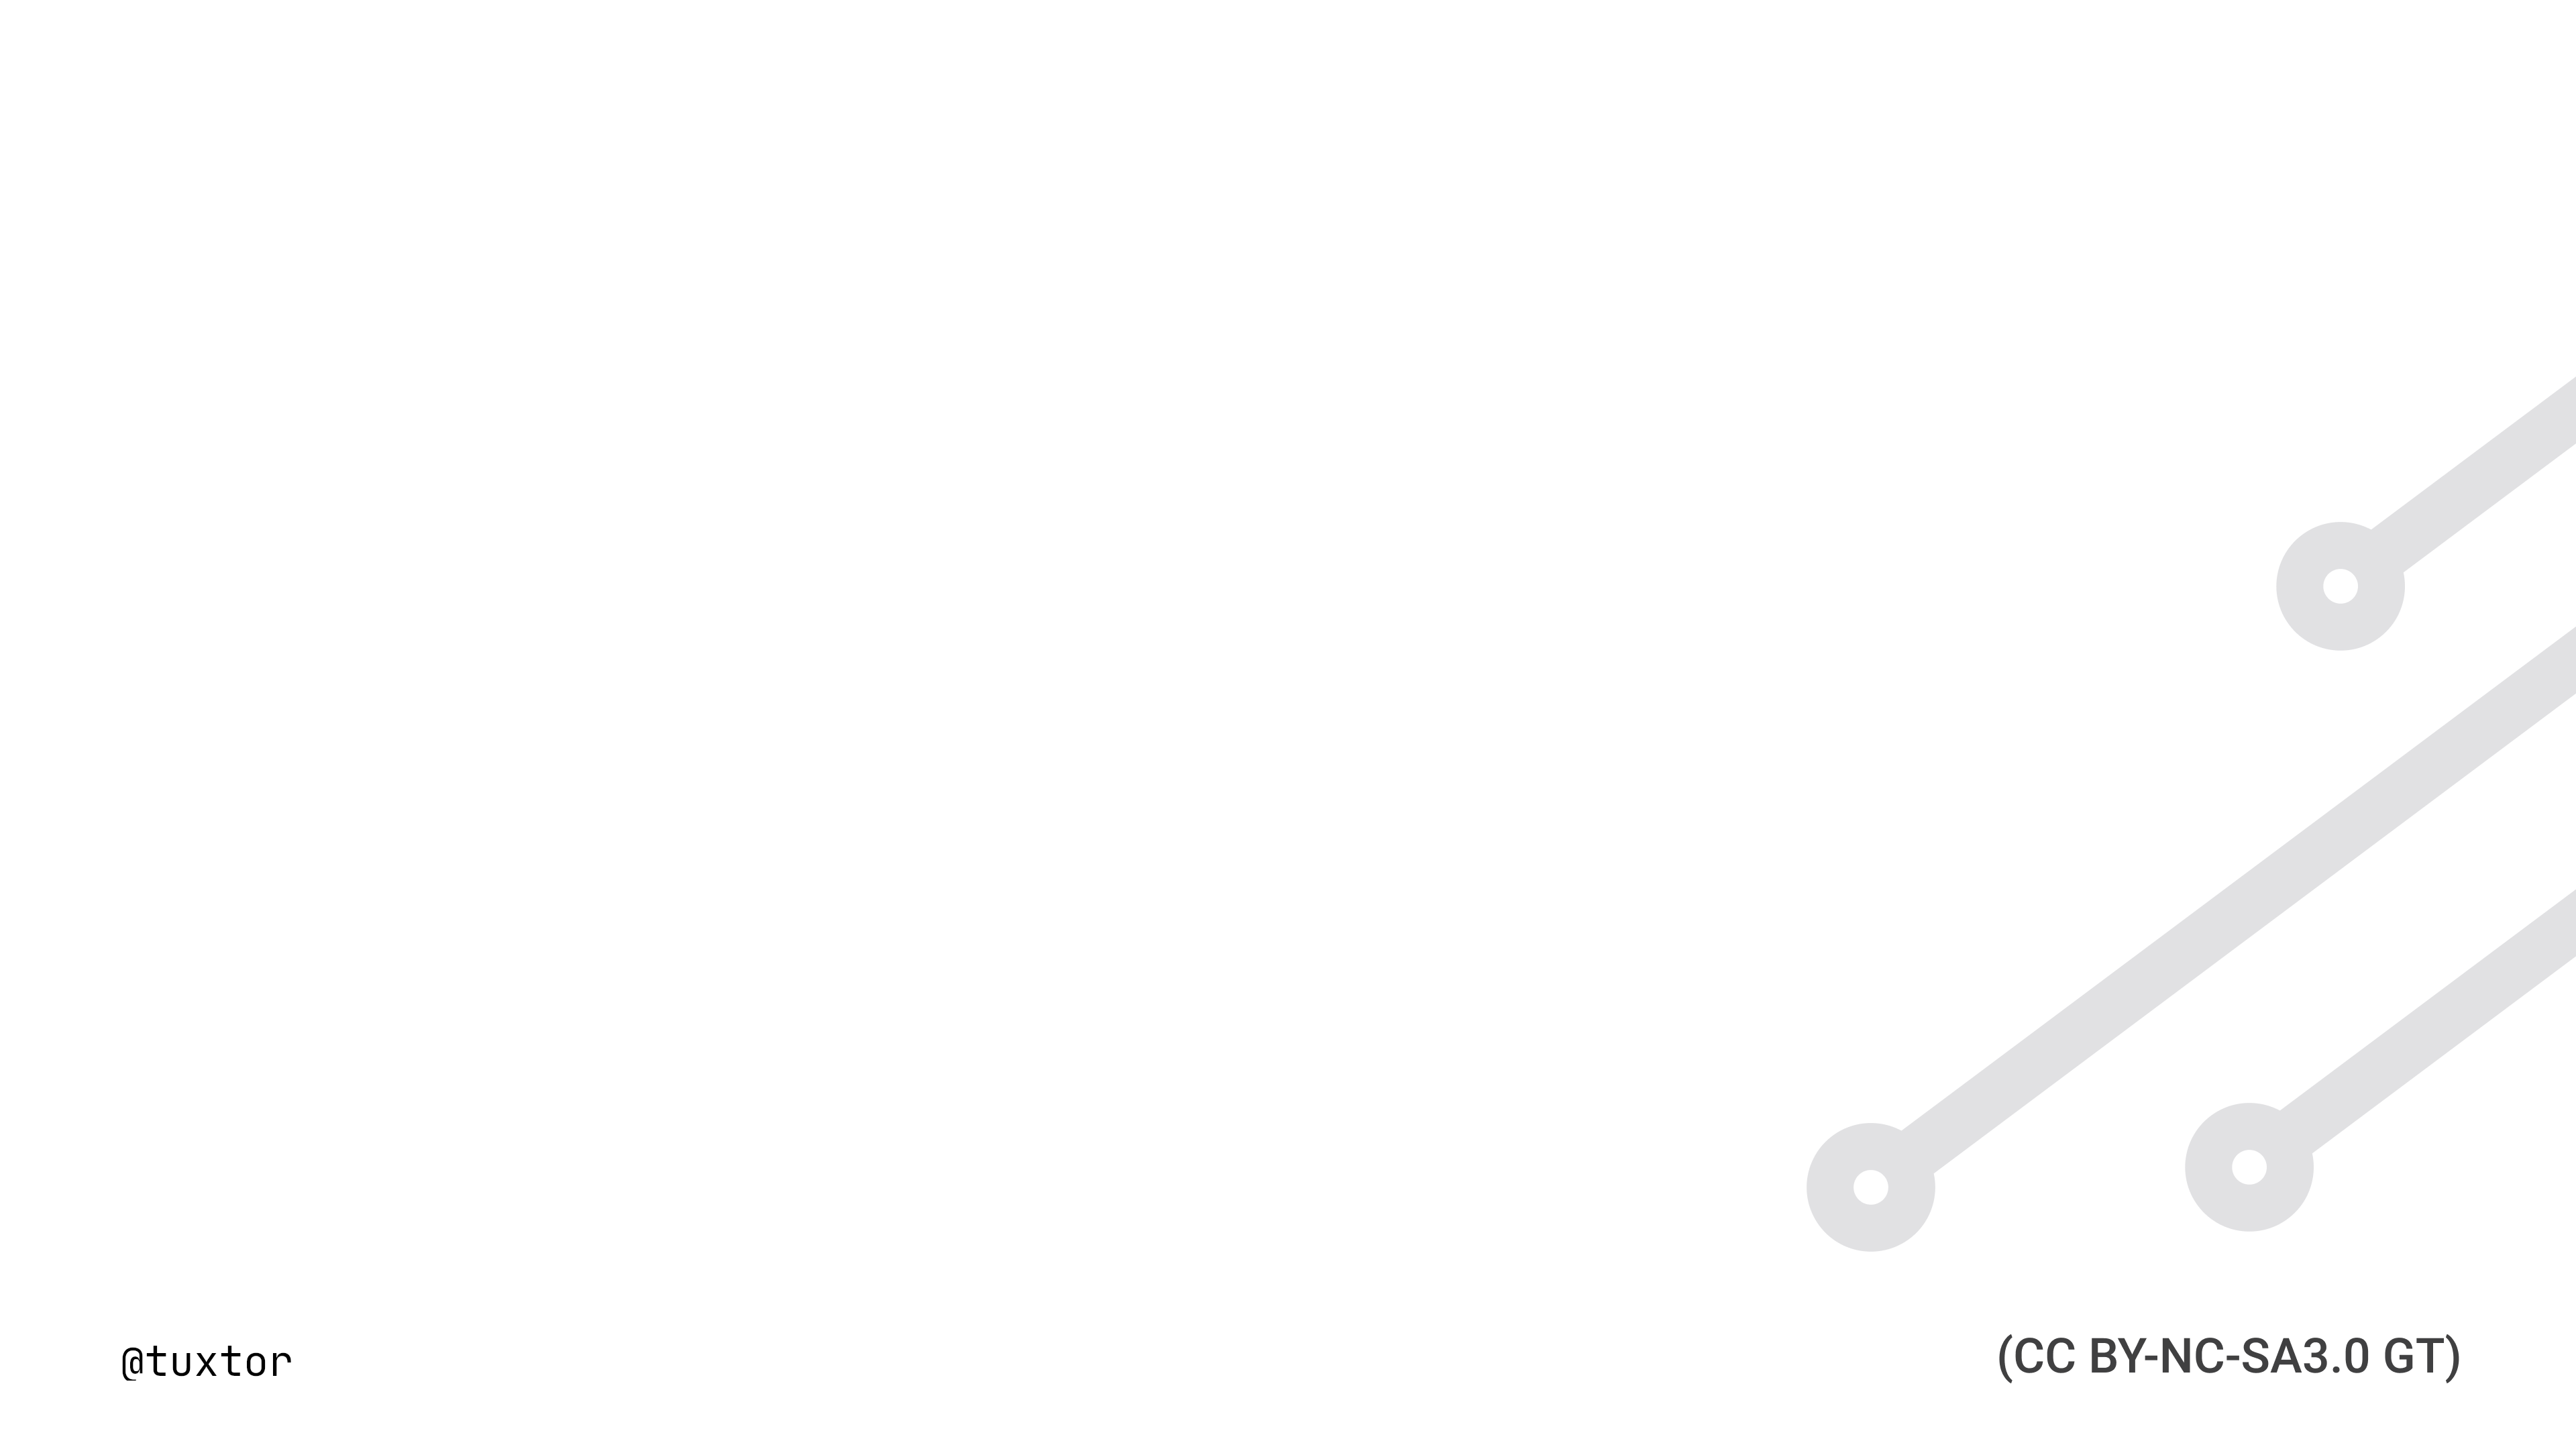
\includegraphics[width=\paperwidth]{Images/fondo}%
}


\title{Microservicios con Jakarta EE y Eclipse MicroProfile}
\author{Víctor Orozco - @tuxtor}
\institute{Academik}
\date{\today}

\begin{document}

{
    \usebackgroundtemplate{
\includegraphics[width=\paperwidth]{Images/portada}}
    \setbeamercolor{frametitle}{fg=red}
    \usebeamercolor[fg]{normal text}
    \frame{\titlepage}
}


\begin{frame}{Java EE}
\begin{exampleblock}{Java EE}
Java Platform, Enterprise Edition (Java EE) is based on the Java SE specification. It represents a \textbf{collaboration between numerous vendors and industry leaders}, and provides the infrastructure support for applications - \textit{IBM}
\end{exampleblock}
\end{frame}

\begin{frame}{Java EE}
\begin{itemize}
\item Especificaciones (Estandares) desarrollados en el Java Community Process -e.g. JPA, CDI, JAX-RS -
\item Implementaciones totales (Glassfish, Weblogic) o parciales (Tomcat, Jetty)
\item TCK (\$\$\$)
\end{itemize}
\end{frame}



\begin{frame}{Java EE 8}
\begin{figure}
	\centering
	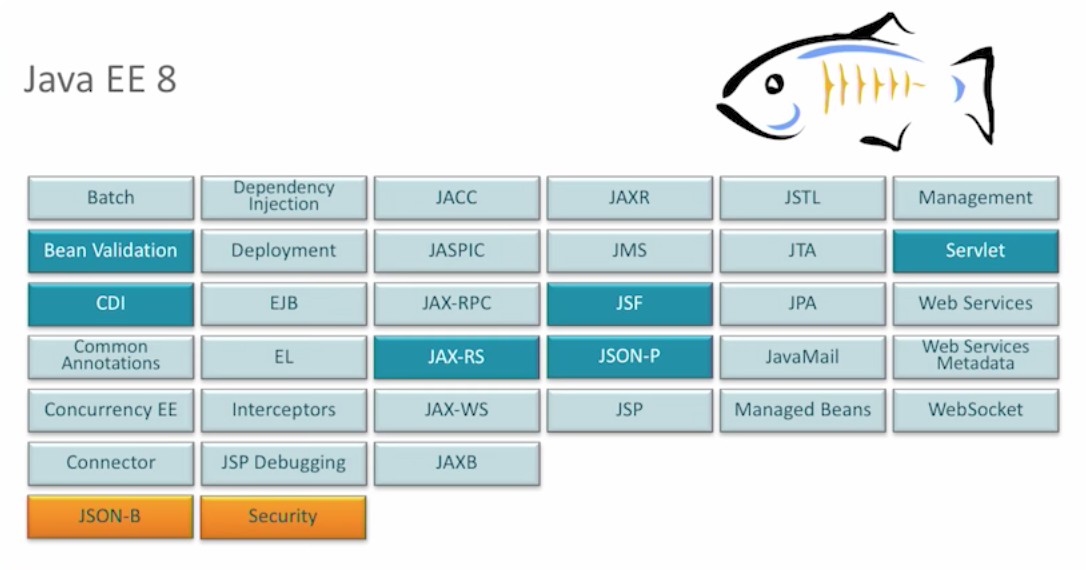
\includegraphics[width=\linewidth]{Images/javaee8}
\end{figure}
\end{frame}

\begin{frame}{Java EE 8}
\begin{figure}
	\centering
	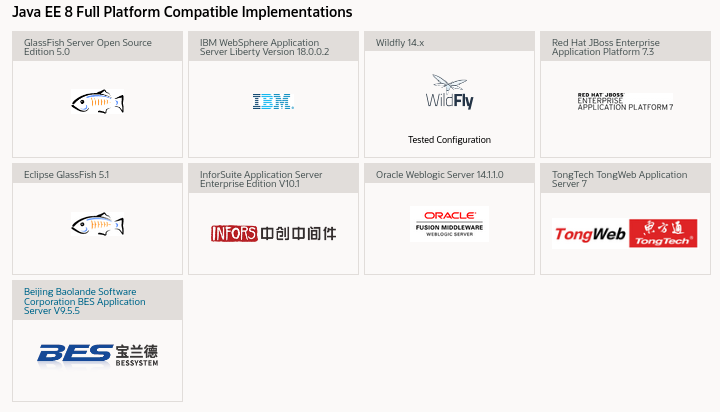
\includegraphics[width=\linewidth]{Images/ee8full}
\end{figure}
\end{frame}

\begin{frame}{Java EE 8}
\begin{figure}
	\centering
	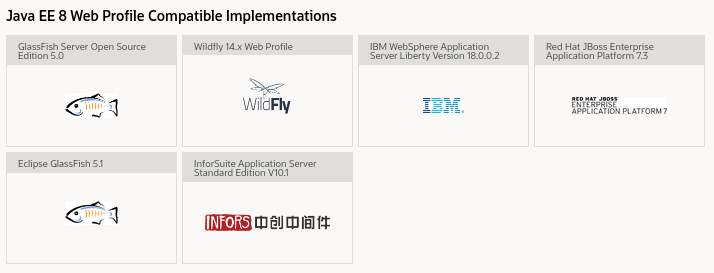
\includegraphics[width=\linewidth]{Images/ee8web}
\end{figure}
\end{frame}

\begin{frame}{Java EE 8}
\begin{alertblock}{Java EE 8}
\begin{itemize}
	\item Mejor integración de JSF con CDI
	\item Mejor integración de JMS con CDI
	\item HTTP/2
	\item JSON-B
	\item Security
	\item \textbf{JAX-RS Reactivo}
\end{itemize}
\end{alertblock}
\end{frame}

\begin{frame}{Java EE - La rebelión}
\begin{columns}
\begin{column}{0.5\textwidth}
\begin{figure}
\centering

\includegraphics[width=\linewidth]{Images/microprofile-logo}
\end{figure}
\end{column}
\begin{column}{0.5\textwidth}  %%<--- here
\begin{figure}
\centering

\includegraphics[width=\linewidth]{Images/guardians}
\end{figure}
\end{column}
\end{columns}
\end{frame}

\begin{frame}{Nace Jakarta EE}
\begin{figure}
	\centering
	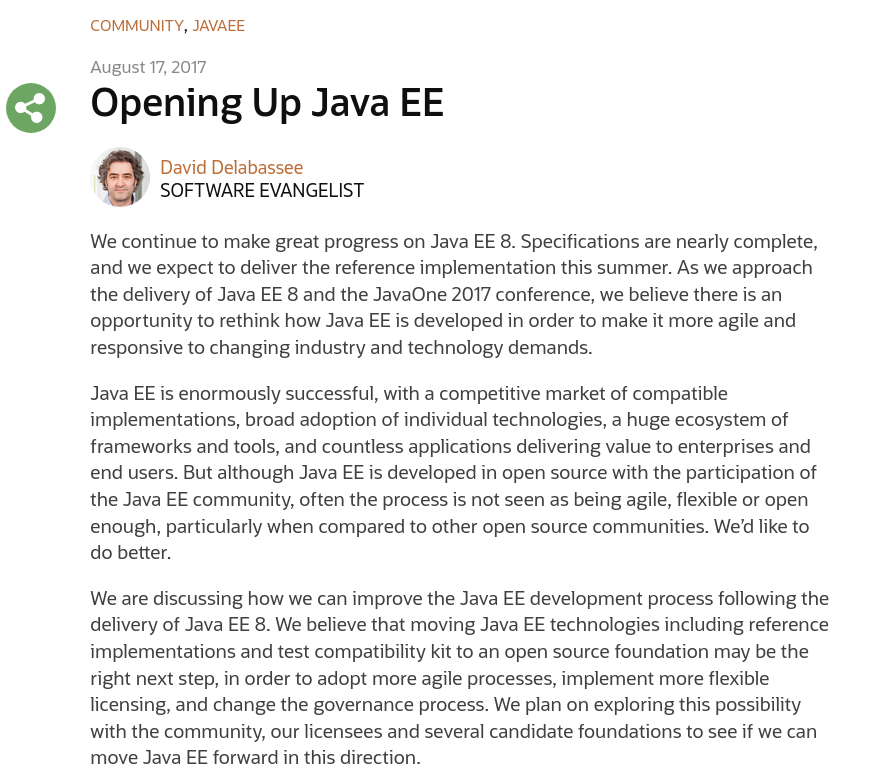
\includegraphics[width=0.7\linewidth]{Images/javaeeopen}
\end{figure}
\end{frame}

\begin{frame}{Java EE - JakartaEE + MicroProfile}
\begin{figure}
	\centering
	
\includegraphics[width=0.7\linewidth]{Images/javaeeevolution}
\end{figure}
\end{frame}


{
    \usebackgroundtemplate{
\includegraphics[width=\paperwidth]{Images/separador}}
    \setbeamercolor{normal text}{fg=white}
    \setbeamercolor{frametitle}{fg=red}
    \usebeamercolor[fg]{normal text}
    \section{Jakarta EE}
}

\begin{frame}{Jakarta EE}
\begin{figure}
	\centering
	
\includegraphics[width=0.7\linewidth]{Images/jakartaee}
\end{figure}
\end{frame}

\begin{frame}{Jakarta EE}
\begin{itemize}
\item Especificaciones (Estandares) desarrollados en la fundación Eclipse -e.g. JPA, CDI, JAX-RS -
\item Implementaciones totales (Glassfish, Weblogic) o parciales (Tomcat, Jetty)
\item TCK (Open Source) y disponibles en Github
\end{itemize}

Cambios más importantes

\begin{itemize}
\item Jakarta EE 8 - Transición hacia Eclipse
\item Jakarta EE 9 - Desde javax.* hacia jakarta.*
\item Jakarta EE 9.1 - Java 11 es el mínimo
\end{itemize}
\end{frame}

\begin{frame}{Jakarta EE}
\begin{figure}
	\centering
	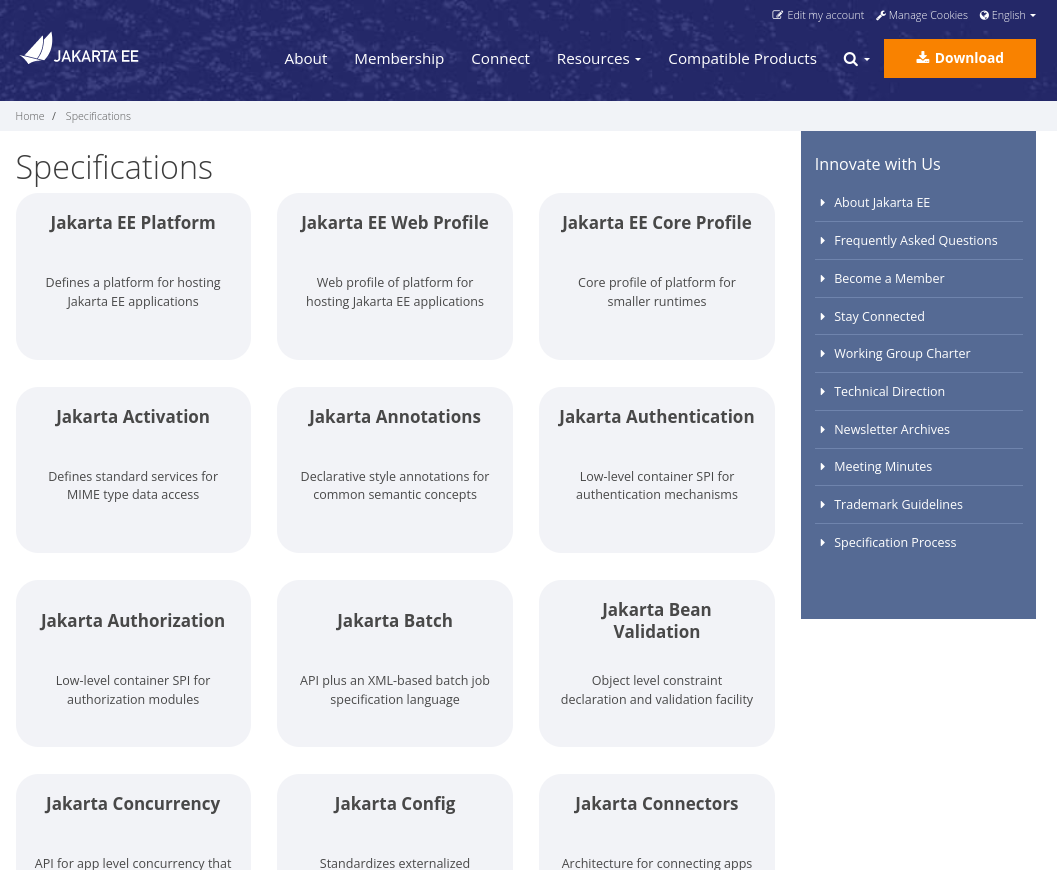
\includegraphics[width=0.7\linewidth]{Images/jakartaeespecs}
\end{figure}
\end{frame}

\begin{frame}{Jakarta EE - Implementaciones}
\begin{figure}
	\centering
	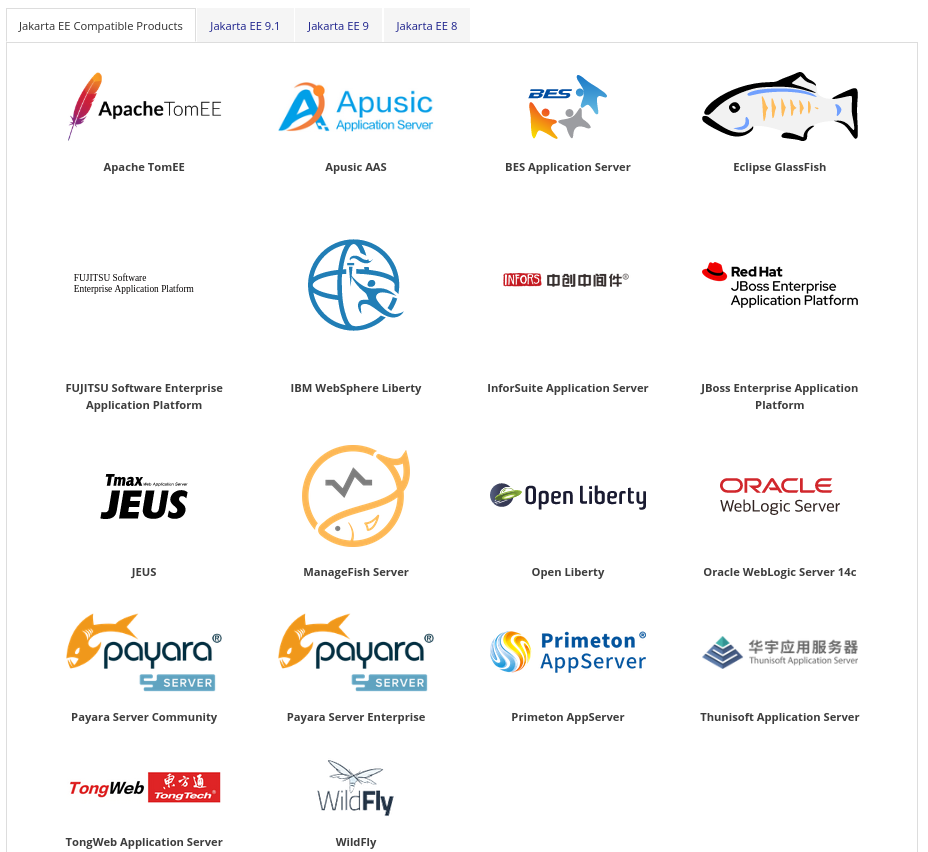
\includegraphics[width=0.7\linewidth]{Images/jakartaeeimplementations}
\end{figure}
\end{frame}
\begin{frame}{Jakarta EE - Migraciones}
\begin{figure}
	\centering
	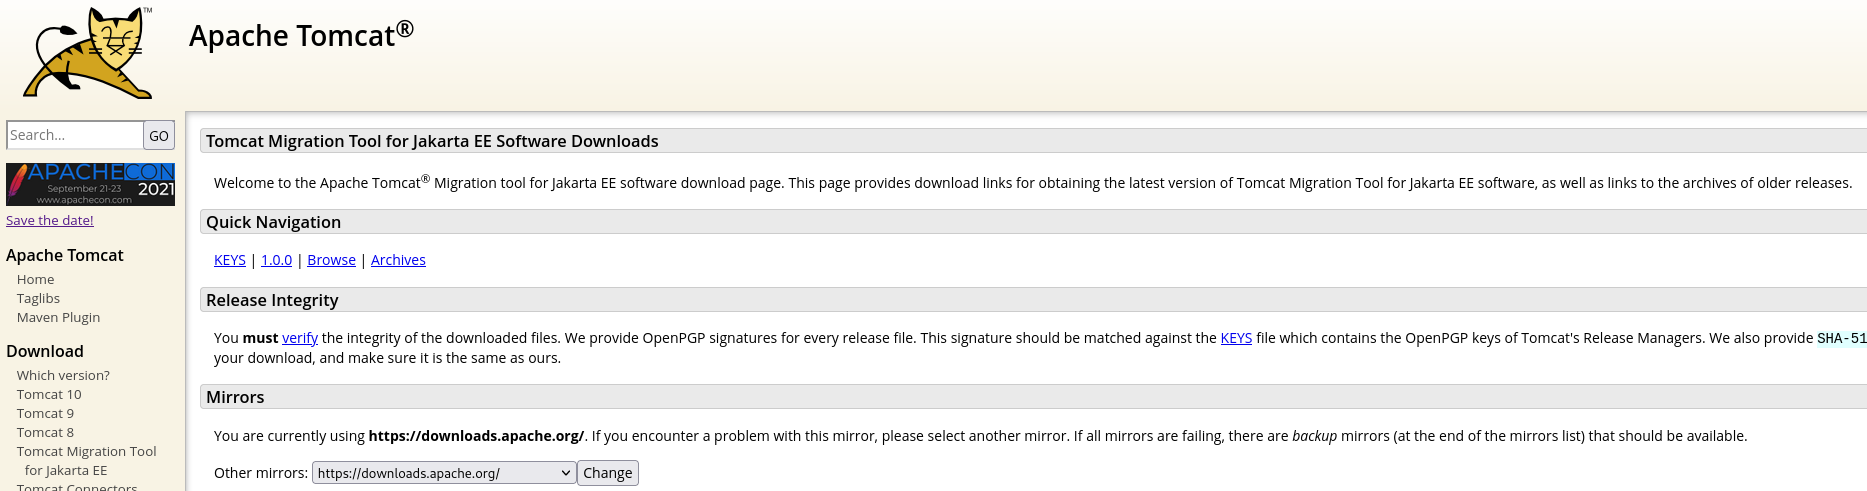
\includegraphics[width=\linewidth]{Images/migration}
\end{figure}
\end{frame}


{
    \usebackgroundtemplate{
\includegraphics[width=\paperwidth]{Images/separador}}
    \setbeamercolor{normal text}{fg=white}
    \setbeamercolor{frametitle}{fg=red}
    \usebeamercolor[fg]{normal text}
    \section{MicroProfile}
}


\begin{frame}{Microservicios - Java EE}
\begin{figure}
	\centering
	
\includegraphics[width=0.9\linewidth]{Images/microprofile-logo}
\end{figure}
\end{frame}

\begin{frame}{Microprofile}
\begin{itemize}
\item Especificaciones (Estandares) desarrollados en la fundación Eclipse -e.g. Fault Tolerance, OpenAPI-
\item Implementaciones con Jakarta EE completo (Payara Micro, Apache TomEE) o unicamente MicroProfile (Oracle Helidon, Red Hat Quarkus )
\item TCK (Open Source) y disponibles en Github
\end{itemize}
\end{frame}

\begin{frame}{Microservicios - Java EE}
\begin{figure}
	\centering
	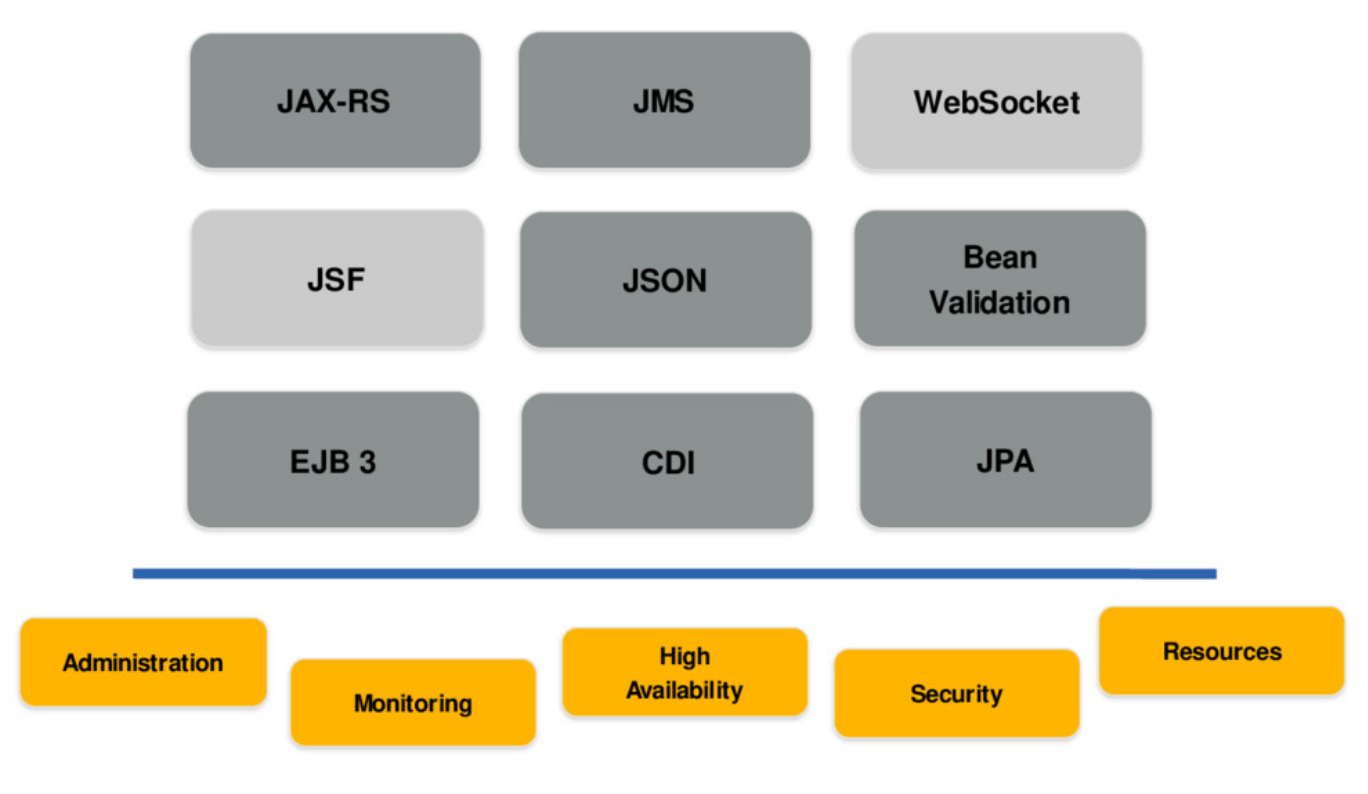
\includegraphics[width=\linewidth]{Images/javaeemicropancake}
\end{figure}
\end{frame}

\begin{frame}{MicroProfile}
\begin{figure}
	\centering
	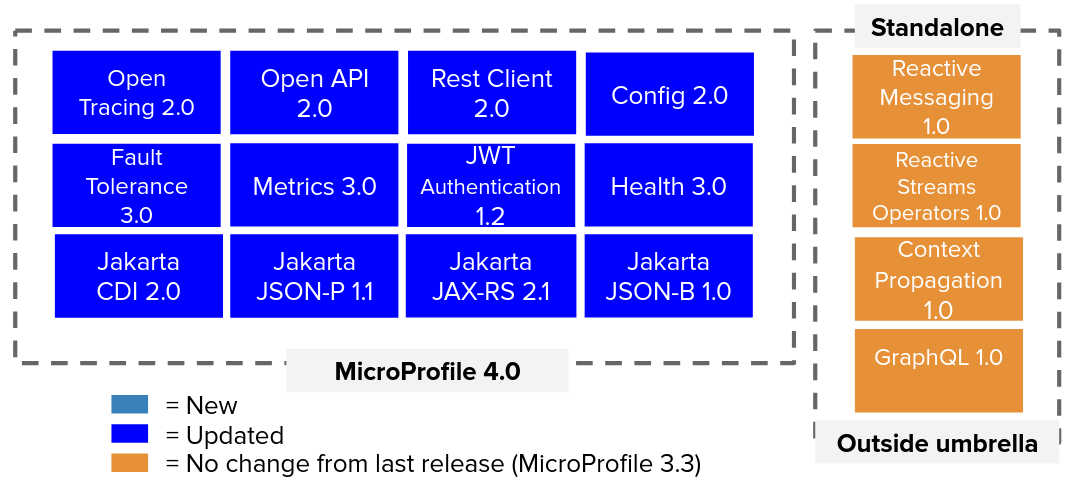
\includegraphics[width=\linewidth]{Images/microprofile}
\end{figure}
\end{frame}

\begin{frame}{MicroProfile}
\begin{figure}
	\centering
	
\includegraphics[width=\linewidth]{Images/microprofileimplementations}
\end{figure}
\end{frame}

\begin{frame}{Cloud Native Java}

Resumen
\begin{itemize}
\item Jakarta EE -WebLogic-
\item MicroProfile -Quarkus, Oracle Helidon-
\item Jakarta EE + MicroProfile -Payara Micro, IBM OpenLiberty-
\item Implementadores -SmallRye, Apache Geronimo, Tomcat, Jetty-
\end{itemize}

Entornos de ejecución
\begin{itemize}
\item Servidores de aplicación
\item Fat-jar/Uber-jar
\item Docker
\end{itemize}
\end{frame}


\begin{frame}{Víctor Orozco}
\begin{columns}[T] % contents are top vertically aligned

	\begin{column}[T]{4cm} % alternative top-align that's better for graphics
		\begin{figure}
			\centering
			
\includegraphics[width=\linewidth]{Images/logos}
		\end{figure}
	\end{column}
	\begin{column}[T]{6cm} % each column can also be its own environment
		\begin{itemize}
			\item vorozco@nabenik.com
			\item \href{https://twitter.com/tuxtor}{@tuxtor}
			\item \href{https://vorozco.com}{https://vorozco.com}
			\item \href{https://tuxtor.shekalug.org}{https://tuxtor.shekalug.org}
		\end{itemize}
		\begin{center}
			
\includegraphics[width=0.1\linewidth]{Images/cclogo}
			\\
			This work is licensed under Creative Commons Attribution-NonCommercial-ShareAlike 3.0 Guatemala (CC BY-NC-SA 3.0 GT).
		\end{center}
	\end{column}
\end{columns}
\end{frame}

\end{document}

